\section{Ziel}
  Ziel des Versuchs ist es, Quarz-Kugeln mittels einer optischen Pinzette einzufangen und zu untersuchen. Es wird daraus die Fallensteifigkeit und die Boltzmann-Konstante bestimmt. Außerdem wird der Transport von Vesikeln durch molekulare Aktin-Myosin-Motoren in Zwiebelzellen untersucht.
\section{Theoretische Grundlagen}
  \subsection{Grundlagen der optischen Falle}
    Da Photonen einen Impuls tragen übt Licht, wenn auch in sehr kleinen Maßen, Kraft aus. Diese Kraft kann zwar nichts in der makroskopischen Welt ausrichten, es ist aber möglich, z.B. durch eine optische Falle, mikroskopisch kleine dielektrische Kugeln zu manipulieren. \cite{ashkin}
    Die Physik hinter dem Einfangen und Bewegen durch eine optische Falle wird als Erstes für Objekte besprochen, welche viel größer sind als die Wellenlänge des verwendeten Lichtes ($d\gg\lambda$).
    Dazu wird die Impulsveränderung des Lichts untersucht. Dieses wird an der Mikrokugel gebrochen und es wird eine Gradientenkraft entgegengesetzt zur Impulsveränderung erzeugt. Die gebrochenen Lichtstrahlen und die entstehenden Gradientenkräfte im Falle von einer zentrierten und nicht zentrierten Mikrokugel sind in Abbildung \ref{fig:Falle} dargestellt.
    \begin{figure}[h]
      \centering
      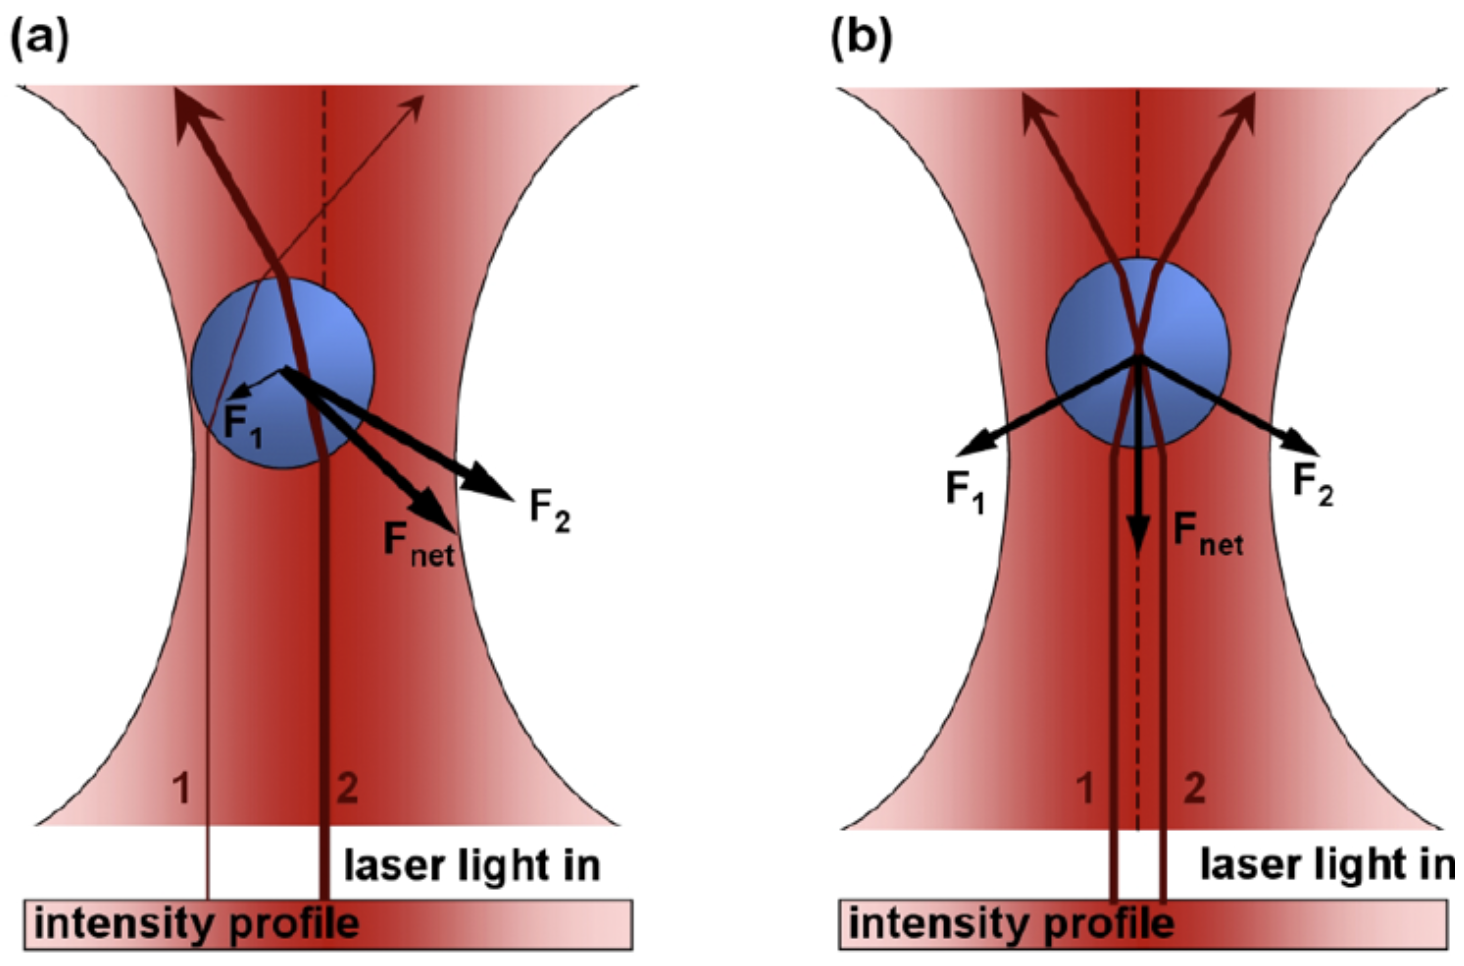
\includegraphics[width = 0.8\textwidth]{pictures/Falle.png}
      \caption{Schematische Skizze der resultierenden Kräfte für eine \textit{a)} nach links ausgelenkte und eine \textit{b)} zentrierte Mikrokugel. Entnommen aus \cite{tu_dortmund_versuchsanleitung_OptischePinzette}}
      \label{fig:Falle}
    \end{figure}
    Da es sich um einen fokussierten Gaußstrahl handelt besitzt das Licht, das aus dem Zentrum gebrochen ist, die größte Intensität und damit die größte Gradientenkraft. Bei einer nach links (rechts) ausgelenkten Kugel entspricht das einer resultierenden Kraft nach rechts (links). Zusammen mit der Streukraft des teilweise reflektierten Lichtes stellt sich so ein Gleichgewicht ein und die Mikrokugel wird im Fallenzentrum festgehalten.

    Für Objekte, die $d\gg\lambda$ nicht erfüllen, gilt die Beschreibung mit der Strahlenoptik nicht mehr. In diesem Fall kommt die Rayleigh-Streuung ins Spiel und das Objekt muss als Dipol betrachtet werden. \cite{neumann}
  \subsection{Fallensteifigkeit und Gleichverteilungstheorem}
    Der Druck $p$, den $N$ Teilchen bei einer Temperatur $T$ in einem Volumen $V$ bewirken, wird durch die ideale Gasgleichung
    \begin{equation}
      p\cdot V = N\cdot k_B\cdot T
    \end{equation}
    beschrieben, wobei $k_B$ die Boltzmann-Konstante ist. Diese Informationen reichen aber noch nicht aus, um $k_B$ zu messen, da keine Schlüsse über die Teilchenanzahl $N$ gezogen werden können.

    Das lässt sich ändern, wenn die Energie eines einzelnen Teilchens mit der Kraftfluktuation kombiniert wird, welche aus den Stößen der Gasteilchen untereinander hervorgeht. Das Äquipartitionstheorem besagt, dass pro Teilchen und Freiheitsgrad die Energie $\frac{1}{2}k_BT$ existiert. Mit dem Vergleich der optischen Falle mit einer Feder mit Federkonstante $k$ ergibt sich für die Energie eines Teilchens, das sich in diesem harmonischen Potential bewegt $\frac{1}{2}k\langle x\rangle^2$. Das Gleichsetzen beider Ausdrücke ergibt
    \begin{equation}
      \frac{1}{2}k\langle x\rangle^2 = \frac{1}{2}k_BT \, ,
    \end{equation}
    wobei $k$ die Fallensteifigkeit der optischen Falle beschreibt und $\langle x\rangle$  die Fluktuation der Teilchenbewegung aufgrund der Brown'schen Bewegung.
  \subsection{Brown'sche Bewegung und spektrale Leistungsverteilungsfunktion}
    Der Einfluss der Brown'schen Bewegung, gemittelt über eine große Anzahl an Teilchen, kann als zufällige Kraft $F(t)$ beschrieben werden. Für eine viskose Bewegung, wie es in der optischen Falle der Fall ist, gilt für die Position $x$ eines Objekts die Bewegungsgleichung
    \begin{equation}
      \beta \dot{x}(t) + kx(t) = F(t)
    \end{equation}
    mit dem hydrodynamischen Zugwiderstand $\beta = 3\pi\eta d$, wobei $d$ den Kugeldurchmesser des Objektes und $\eta$ die Viskosität des verwendeten Mediums beschreibt. Diese Bewegungsgleichung kann für alle drei Raumrichtungen mit drei unterschiedlichen Fallensteifigkeiten $k_x$, $k_y$ und $k_z$ aufgestellt werden.

    Nach dem Wiener-Khinchin-Theorem gilt für das spektrale Leistungsspektrum
    \begin{equation}
      S_{xx}(f) = \sqrt{\frac{k_B T}{\pi^2\beta(f^2+f_0^2)}}
      \label{eqn:Leistung}
    \end{equation}
    mit der sogenannten "Roll-Off-Frequenz"
    \begin{equation}
      f_0 = \frac{k}{2\pi\beta}
      \label{eqn:Roll}
    \end{equation}
    aus welcher die Fallensteifigkeit $k$ der optischen Falle ermittelt werden kann.
  \subsection{Molekulare Motoren in der Mikrobiologie}
    In Zellen werden Informationen und verschiedene Stoffe mit Hilfe von Organellen/Vesikeln transportiert. Diese sind meistens $\sim 1\mu\text{m}$ groß und bewegen sich entlang von Aktin-Kanälen. Diese Bewegung wird von einem Myosin-Motor-Protein verrichtet, welches sich praktisch an den Aktin-Kanälen 'entlanghangeln'. Dieser Prozess ist in Abbildung \ref{fig:Motor} schematisch verdeutlicht.
    \begin{figure}[h]
      \centering
      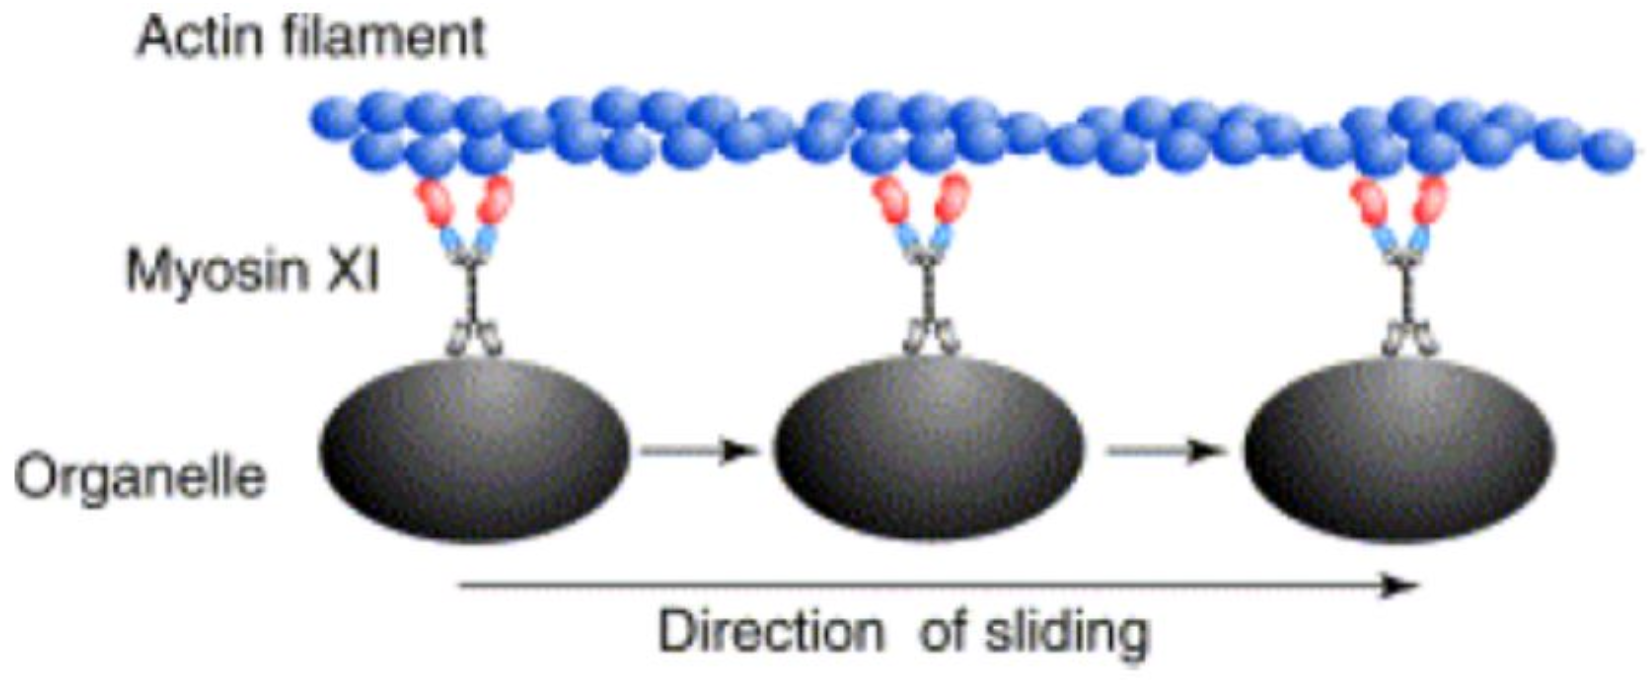
\includegraphics[width = 0.8\textwidth]{pictures/Motor.png}
      \caption{Bewegung eines Vesikels 'durch' Aktin-Kanäle mit Hilfe von Myosin-Motoren. Entnommen aus \cite{tu_dortmund_versuchsanleitung_OptischePinzette}}
      \label{fig:Motor}
    \end{figure}
    